\documentclass[12pt]{article}

\usepackage[margin=1in]{geometry}
\usepackage{amsmath, amssymb, amsthm}
\usepackage{graphicx}
\usepackage{booktabs}
\usepackage{hyperref}
\usepackage{natbib}
\usepackage{setspace}
\usepackage{caption}
\usepackage{float}

\onehalfspacing

\title{Preference Diversity and Evolutionary Stability\\
in Concave Public Goods Games:\\
Homo Oeconomicus, Homo Kantiensis, and Pure Altruists}
\author{}
\date{}

\begin{document}

\maketitle

\begin{abstract}
We study the evolutionary stability of three preference types---Homo Oeconomicus (pure self-interest), Homo Kantiensis (pure Kantian morality), and Pure Altruist---in a concave public goods game with assortative matching. Drawing on the framework of \citet{AlgerWeibull2013}, we introduce an assortativity index $\sigma \in [0,1]$ that governs the probability of like-type encounters and derive closed-form equilibrium strategies for each type. Replicator-dynamic simulations reveal a phase transition at $\sigma \approx 0.35$: below this threshold, the Homo Oeconomicus free-rider dominates; above it, the Kantian type prevails. The Pure Altruist is eliminated under \emph{all} matching regimes because its equilibrium strategy systematically exceeds the social optimum, incurring costs that outweigh the public benefit. A central insight is the symmetry between under- and over-contribution: both Homo Oeconomicus and Pure Altruist deviate from the social optimum in opposite directions, and it is precisely the type that \emph{coincides} with the social optimum---Homo Kantiensis---that proves evolutionarily robust at high assortativity.
\end{abstract}

%-----------------------------------------------------------------------
\section{Introduction}
%-----------------------------------------------------------------------

A long-standing question in evolutionary economics and biology is which preference types survive selection pressure in strategic environments. \citet{AlgerWeibull2013} show that when individuals are matched assortatively, the evolutionarily stable type is \emph{homo moralis}---a preference that blends self-interest with a Kantian component weighted by the assortativity index $\sigma$. At the extremes, $\sigma = 0$ selects pure self-interest and $\sigma = 1$ selects the pure Kantian type.

The present paper instantiates this framework in the specific context of a concave public goods game and examines \emph{three discrete preference types} that correspond to the two extremes and a third benchmark: (i) Homo Oeconomicus ($\kappa = 0$), (ii) Homo Kantiensis ($\kappa = 1$), and (iii) the Pure Altruist, whose utility function is the opponent's material payoff. The concave payoff structure is chosen deliberately: unlike the linear public goods game, it produces distinct interior equilibrium strategies for all three types and thereby separates their fitness profiles in a non-degenerate way.

We proceed as follows. Section~\ref{sec:model} presents the game, the three preference types, and the replicator dynamics. Section~\ref{sec:results} reports simulation results under four representative values of $\sigma$. Section~\ref{sec:discussion} discusses the mechanisms behind each type's evolutionary fate. Section~\ref{sec:conclusion} concludes.

%-----------------------------------------------------------------------
\section{Model}\label{sec:model}
%-----------------------------------------------------------------------

\subsection{The Concave Public Goods Game}

A \textbf{game} describes a situation in which multiple agents make decisions and each agent's outcome depends on the choices of all participants. In the present model, each interaction is a two-player game in which both players simultaneously choose a contribution level $x \in [0,1]$ to a shared public good. Higher total contributions generate more public benefit, but each unit contributed imposes a private cost on the contributor. This creates a \textbf{social dilemma}: collectively, high contributions are efficient, but individually, each player has an incentive to free-ride on the other's effort.

Formally, player $i$'s material payoff is given by the following \textbf{concave public goods game}:
\begin{equation}
    \pi(x_i, x_j) = r(x_i + x_j) - \frac{r(x_i + x_j)^2}{2} - x_i,
    \label{eq:pgg}
\end{equation}
with parameter $r = 3$ (public good return rate; $r > 1$ is required for social value of cooperation). The term $-r(x_i+x_j)^2/2$ captures a congestion effect: marginal returns to the public good are decreasing in total contributions. The term $-x_i$ is the private cost of contributing.

Unlike the linear public goods game, this concave specification ensures that the social optimum lies at an interior point, and that all three preference types have distinct equilibrium contributions---properties that are essential for a non-degenerate comparison.

The social dilemma persists: at any interior total contribution $x_i + x_j$, the marginal return to contributing is $r - r(x_i+x_j) < 1$ once total contributions are sufficiently large, so the private cost exceeds the private return from one's own contribution.

\subsection{Preference Types and Equilibrium Strategies}

Each agent maximises a \textbf{utility function}---the objective she genuinely cares about---which need not coincide with material payoff $\pi$. The three types and their utility functions are listed in Table~\ref{tab:types}. Their equilibrium strategies are derived in Section~\ref{sub:equilibrium}.

\begin{table}[H]
    \centering
    \caption{Preference types and equilibrium strategies}
    \label{tab:types}
    \begin{tabular}{llll}
        \toprule
        Label & Type & Utility function & Equilibrium strategy \\
        \midrule
        H & Homo Oeconomicus & $u_H = \pi(x, y)$ & $x_H^* = \dfrac{r-1}{2r}$ \\[8pt]
        K & Homo Kantiensis  & $u_K = \pi(x, x)$ & $x_K^* = \dfrac{2r-1}{4r}$ \\[8pt]
        A & Pure Altruist    & $u_A = \pi(y, x)$ & $x_A^* = \dfrac{1}{2}$ \\
        \bottomrule
    \end{tabular}
\end{table}

\paragraph{Homo Oeconomicus (H).} Maximises own material payoff $\pi(x,y)$. At any fixed opponent strategy $y$, H chooses $x$ to maximise $\pi(x,y)$. This corresponds to the standard Nash best-response and represents pure self-interest with no consideration of the opponent's welfare.

\paragraph{Homo Kantiensis (K).} Applies the Kantian categorical imperative: chooses the contribution $x$ that maximises the outcome \emph{if everyone were to choose the same $x$}, i.e., maximises $\pi(x,x)$. As shown below, this strategy coincides exactly with the social optimum in the concave public goods game.

\paragraph{Pure Altruist (A).} Maximises the \emph{opponent's} material payoff $\pi(y,x)$, choosing the contribution that is best for the other player, irrespective of own welfare. This represents the polar opposite of Homo Oeconomicus.

\subsection{Derivation of Equilibrium Strategies}\label{sub:equilibrium}

An \textbf{equilibrium strategy} is the contribution level at which an agent cannot increase her own utility by unilaterally deviating, given the opponent's strategy. For H, this is the standard Nash equilibrium of the material payoff game. For K and A, the utility function differs from $\pi$, so their equilibria are more precisely \textbf{type-specific best responses}---optimal solutions under each type's own preferences---rather than Nash equilibria of the material payoff game. The solution method is uniform: differentiate the utility function with respect to $x$, set the derivative to zero (first-order condition, FOC), and impose symmetry ($x = y$).

\paragraph{Homo Oeconomicus.}
Writing out the utility function explicitly:
$$u_H = \pi(x,y) = r(x+y) - \frac{r(x+y)^2}{2} - x.$$
The FOC with respect to $x$:
$$\frac{\partial u_H}{\partial x} = r - r(x+y) - 1 = 0 \implies x + y = \frac{r-1}{r}.$$
The $-1$ term arises from the private cost $-x$, which acts as a brake on contributions. Imposing the symmetric Nash condition $x = y$:
$$x_H^* = \frac{r-1}{2r} = \frac{1}{3} \quad (r=3).$$

\paragraph{Homo Kantiensis.}
The Kantian acts as if the opponent also plays $x$, so:
$$u_K = \pi(x,x) = r(2x) - \frac{r(2x)^2}{2} - x = 2rx - 2rx^2 - x.$$
FOC:
$$\frac{\partial u_K}{\partial x} = 2r - 4rx - 1 = 0 \implies x_K^* = \frac{2r-1}{4r} = \frac{5}{12} \approx 0.417 \quad (r=3).$$
This is the \textbf{social optimum}: the contribution level that maximises total welfare $2\pi(x,x)$. The Kantian rule is therefore equivalent to maximising aggregate surplus in this game.

\paragraph{Pure Altruist.}
The altruist maximises the opponent's payoff. Writing $\pi(y,x)$ with the altruist's own contribution as the second argument:
$$u_A = \pi(y,x) = r(y+x) - \frac{r(y+x)^2}{2} - y.$$
The private cost term is $-y$ (the \emph{opponent's} cost), so it vanishes when differentiating with respect to $x$:
$$\frac{\partial u_A}{\partial x} = r - r(y+x) = 0 \implies x = 1 - y.$$
No $-1$ term appears because the altruist's own contribution cost does not enter her utility. Imposing symmetry $x = y$: $x_A^* = 1/2$ (independent of $r$).

The strict ordering
\begin{equation}
    x_H^* = \frac{r-1}{2r} \;<\; x_K^* = \frac{2r-1}{4r} \;<\; x_A^* = \frac{1}{2}
\end{equation}
holds for all $r > 1$. The altruist's contribution exceeds the social optimum $x_K^*$, implying that she bears costs beyond the socially efficient level.

Figure~\ref{fig:strategies} displays the three objective functions and their optima, as well as material payoffs as a function of the opponent's strategy.

\begin{figure}[H]
    \centering
    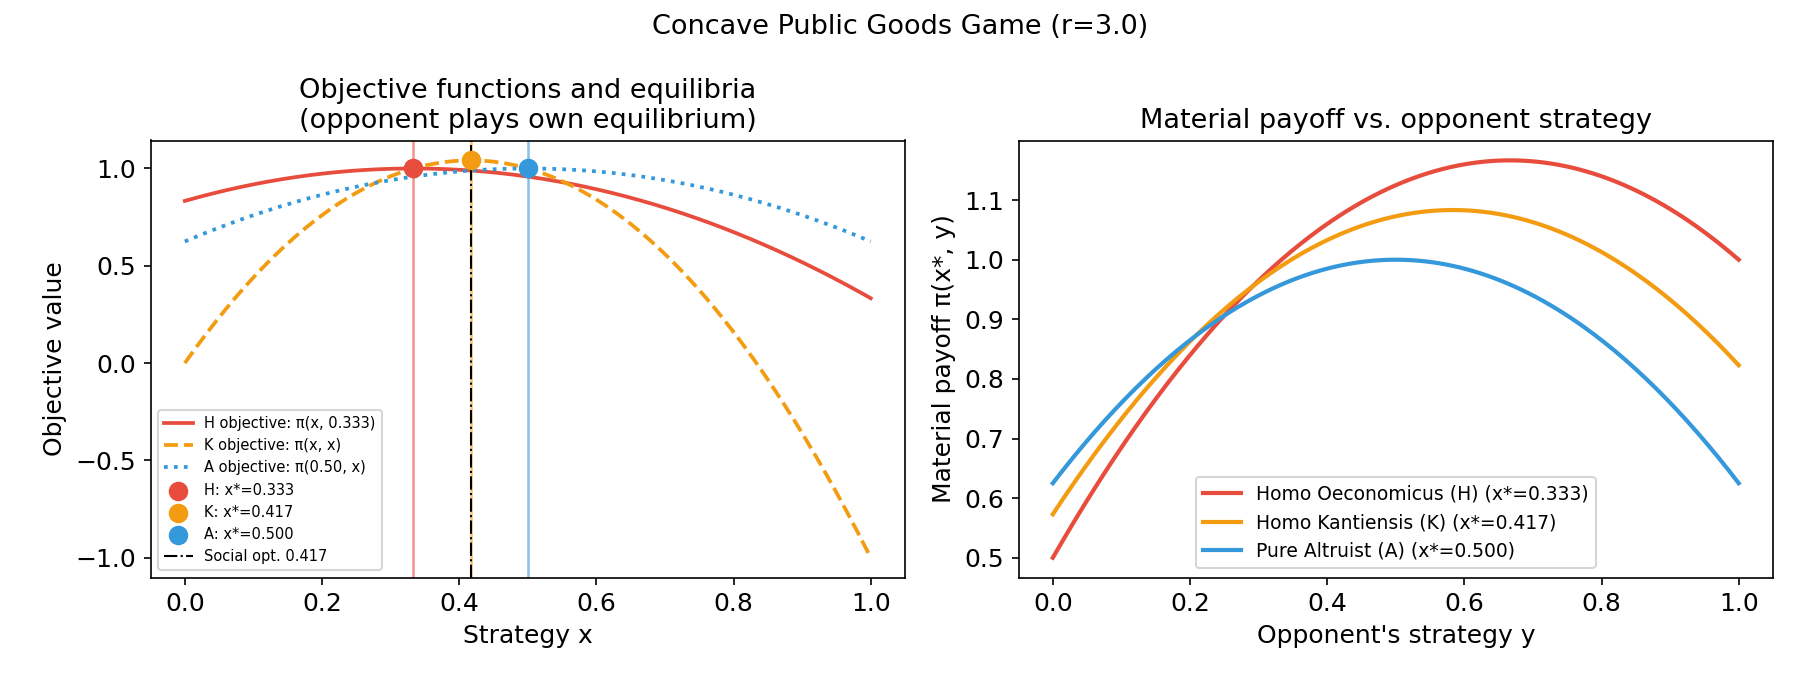
\includegraphics[width=\textwidth]{Code/pgg_strategies.png}
    \caption{Left: objective functions and equilibrium contributions (vertical lines) for each type. H maximises $\pi(x, x_H^*)$ (opponent fixed at H's equilibrium); K maximises $\pi(x,x)$ (Kantian criterion); A maximises $\pi(x_A^*, x)$ (opponent's payoff, own contribution on horizontal axis). Each curve peaks at the corresponding equilibrium. Right: material payoff $\pi(x^*, y)$ for each type as the opponent's strategy varies. Homo Kantiensis achieves the highest material payoff over most of the opponent-strategy range.}
    \label{fig:strategies}
\end{figure}

\subsection{Assortative Matching and Fitness}

Following \citet{AlgerWeibull2013}, we introduce the \textbf{assortativity index} $\sigma \in [0,1]$: in each period, an individual meets a like-type partner with probability $\sigma$ and a randomly drawn partner from the population with probability $1-\sigma$. The average material payoff (fitness) of type $i$ is:
\begin{equation}
    f_i = \sigma \cdot \pi(x_i^*, x_i^*) + (1-\sigma) \sum_j s_j \cdot \pi(x_i^*, x_j^*),
    \label{eq:fitness}
\end{equation}
where $s_j$ is the population share of type $j$ and $x_i^*$ is type $i$'s fixed equilibrium strategy.

The parameter $\sigma$ can be interpreted as a measure of \textbf{social structure}: $\sigma \approx 0$ corresponds to a large, anonymous population in which interactions are essentially random, while high $\sigma$ describes a setting with strong in-group clustering or repeated interactions within tight communities.

\textbf{Fitness} $f_i$ measures the \emph{expected material payoff} of type $i$ in the current population. In the replicator dynamics framework, fitness determines reproductive success---types with above-average fitness expand their population share, and those with below-average fitness contract. Note that fitness is measured in \emph{material payoff} $\pi$, not in each type's own utility: evolution selects on outcomes, not intentions.

\subsection{Population Dynamics: Replicator Equation}

We model the population as undergoing a constant-size replacement process: in each period, a number of individuals die and are replaced by new entrants drawn from the current type distribution. Death probability is proportional to \emph{relative fitness disadvantage}. The logic proceeds in three steps:
\begin{enumerate}
    \item \textbf{Fitness} determines each type's relative reproductive success.
    \item \textbf{Fitness differentials} drive population replacement: types with above-average fitness are over-represented among survivors, below-average types are under-represented.
    \item In the continuous limit, this replacement process converges to the \textbf{standard replicator equation}.
\end{enumerate}

Formally:
\begin{equation}
    s_i(t+1) = s_i(t) + s_i(t)\,\bigl(f_i(t) - \bar{f}(t)\bigr),
    \quad \bar{f}(t) = \sum_j s_j(t)\,f_j(t).
\end{equation}
Types with fitness above the population mean $\bar{f}$ gain share; those below lose share; shares always sum to one.

Simulation parameters: $N = 800$ generations; initial equal shares ($s_H = s_K = s_A = 1/3$); $\sigma \in \{0.0,\, 0.25,\, 0.40,\, 0.80\}$.

%-----------------------------------------------------------------------
\section{Results}\label{sec:results}
%-----------------------------------------------------------------------

\subsection{Fitness Structure}

Before examining dynamics, we characterise the fitness ordering as a function of $\sigma$ at the equal-share initial condition (Figure~\ref{fig:fitness}).

\begin{figure}[H]
    \centering
    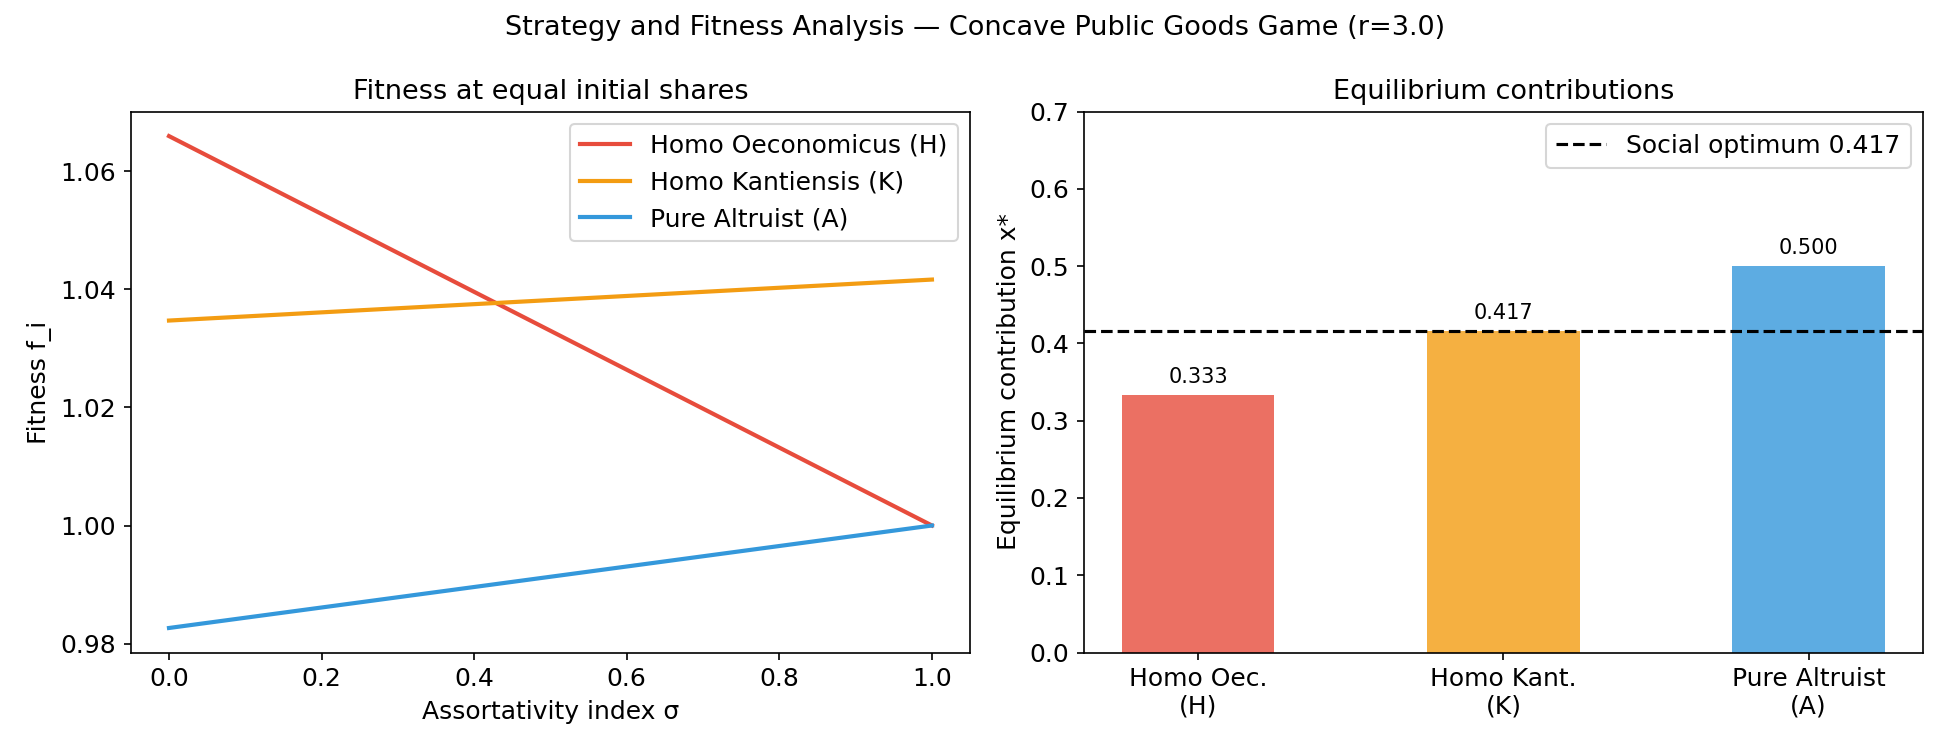
\includegraphics[width=\textwidth]{Code/pgg_fitness.png}
    \caption{Left: fitness of each type at equal initial shares ($s_H = s_K = s_A = 1/3$) as a function of the assortativity index $\sigma$. Right: equilibrium contributions for each type; dashed line marks the social optimum.}
    \label{fig:fitness}
\end{figure}

Three features stand out:
\begin{itemize}
    \item \textbf{Homo Oeconomicus (H):} fitness is highest at $\sigma = 0$ (free-riding pays in anonymous matching) and decreases monotonically as $\sigma$ rises. As more interactions occur within type, H increasingly meets other H types, and the mutually low contributions reduce the public good, lowering fitness.

    \item \textbf{Homo Kantiensis (K):} fitness increases monotonically in $\sigma$. Assortative matching causes K types to meet each other more often; when two K types interact, both contribute at the social optimum, producing maximum joint surplus.

    \item \textbf{Pure Altruist (A):} fitness is strictly below K at \emph{every} $\sigma$, and below H at low $\sigma$. The reason is structural: $x_A^* = 0.5 > x_K^* \approx 0.417 = x_{\text{soc}}^*$. In the concave game, over-contributing beyond the social optimum raises others' payoffs by less than it costs the contributor. A therefore bears a self-inflicted efficiency loss relative to K.
\end{itemize}

This fitness structure directly predicts the dynamic outcome: A is eliminated everywhere; the H-K contest is decided by $\sigma$.

\subsection{Population Dynamics}

Figure~\ref{fig:population} shows the share trajectories over 800 generations for four values of $\sigma$.

\begin{figure}[H]
    \centering
    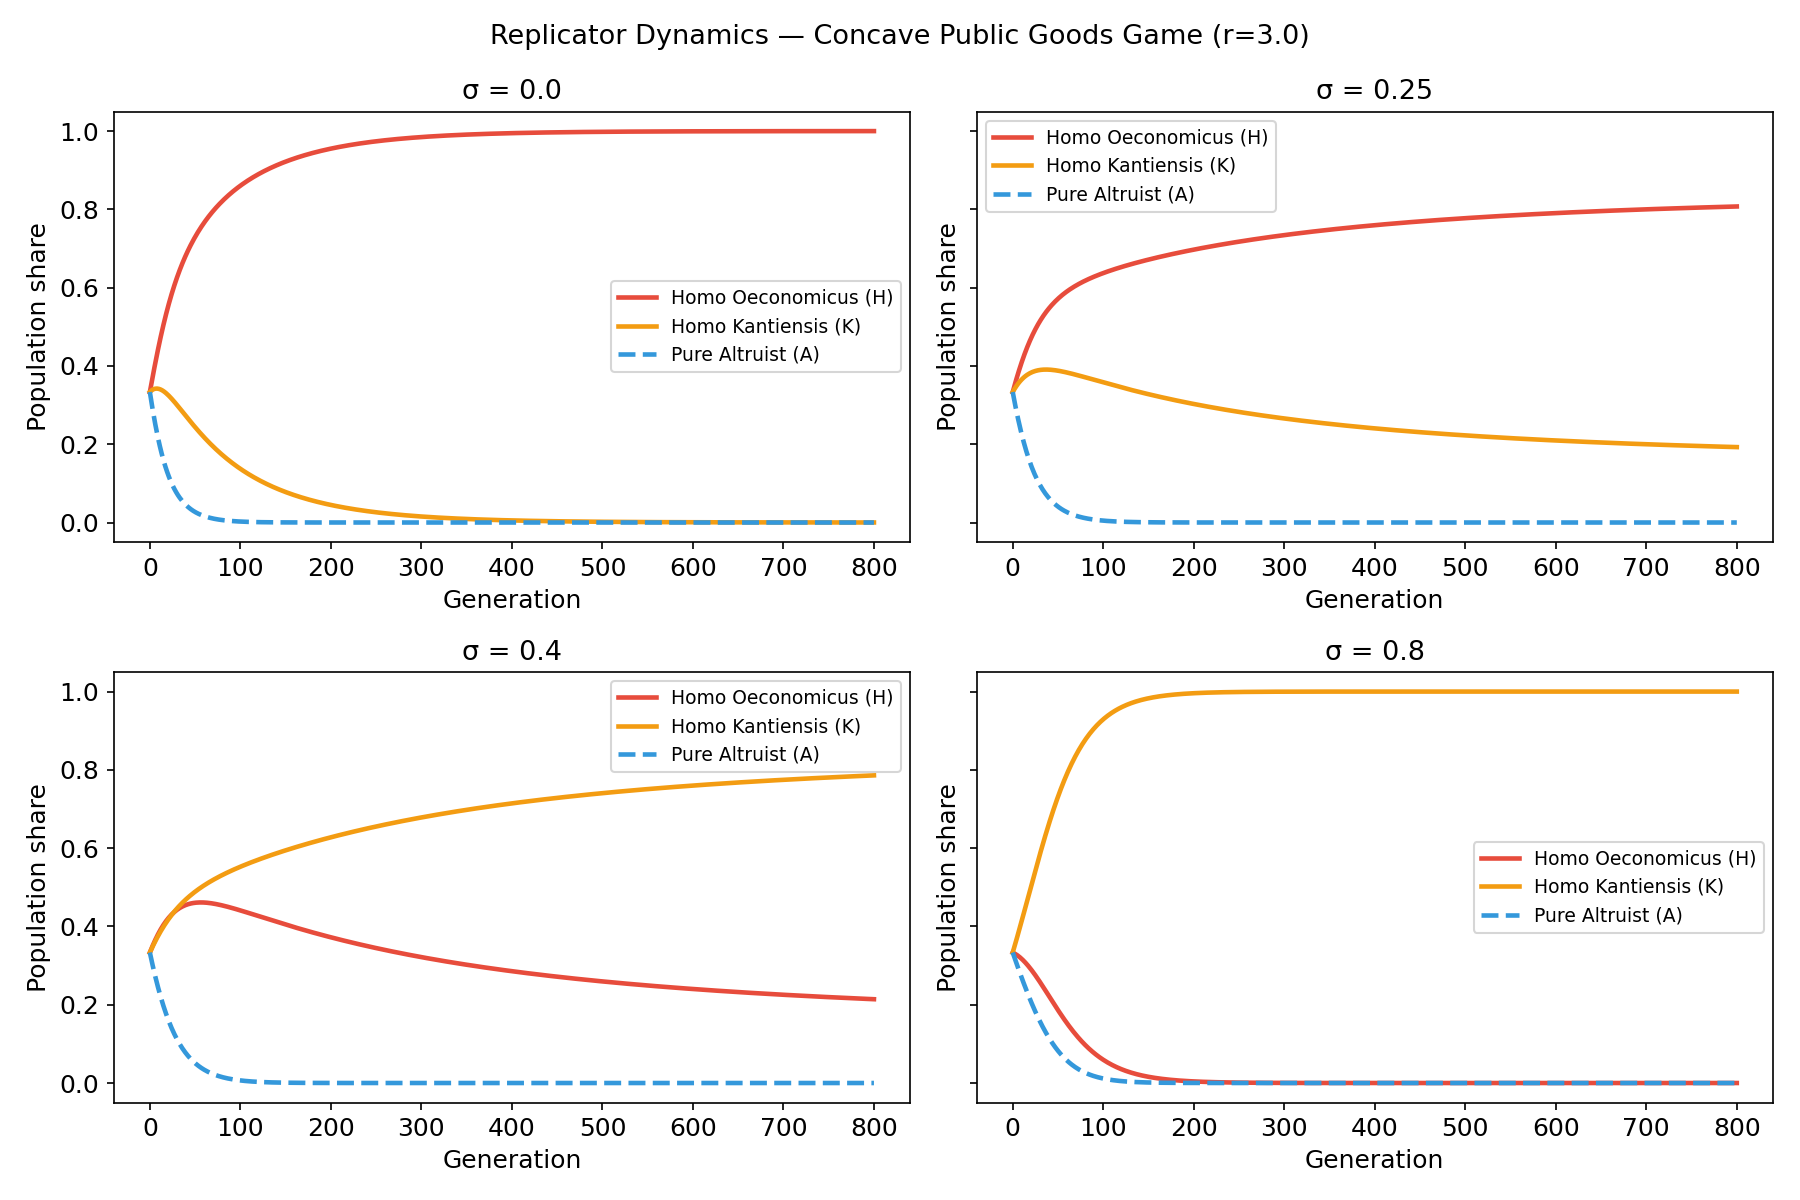
\includegraphics[width=\textwidth]{Code/pgg_population.png}
    \caption{Replicator dynamics for three preference types under four assortativity regimes (800 generations, equal initial shares).}
    \label{fig:population}
\end{figure}

\paragraph{$\sigma = 0.0$ (pure random matching).} H dominates within approximately 200 generations, reaching 100\% share. K and A are eliminated. Free-riding is universally advantageous when matches are anonymous.

\paragraph{$\sigma = 0.25$ (low assortativity).} H still dominates, stabilising near 63\% while K stabilises near 37\%. A reaches zero. Occasional like-type encounters give K a foothold, but the free-riding advantage is not yet overcome.

\paragraph{$\sigma = 0.40$ (transition regime).} An \textbf{interior equilibrium} emerges: K stabilises near 79\%, H near 21\%, A at zero. Note the transient dynamics: H maintains an early advantage for roughly the first 100 generations (random-match free-riding still pays in a mixed population), before K accumulates sufficient critical mass to overtake. This $\sigma$ lies above the phase transition threshold; K achieves majority share for the first time, but both types coexist.

\paragraph{$\sigma = 0.80$ (high assortativity).} K dominates within approximately 150 generations, reaching 100\%. Assortative matching makes K's Kantian strategy overwhelmingly advantageous: nearly all interactions are K-K encounters at the social optimum. H's free-riding incentive essentially disappears because the marginal random partner is almost always a K type playing a high contribution.

\subsection{Phase Diagram: Steady-State Composition}

Figure~\ref{fig:phase} sweeps $\sigma$ continuously from 0 to 1 and reports the steady-state type composition.

\begin{figure}[H]
    \centering
    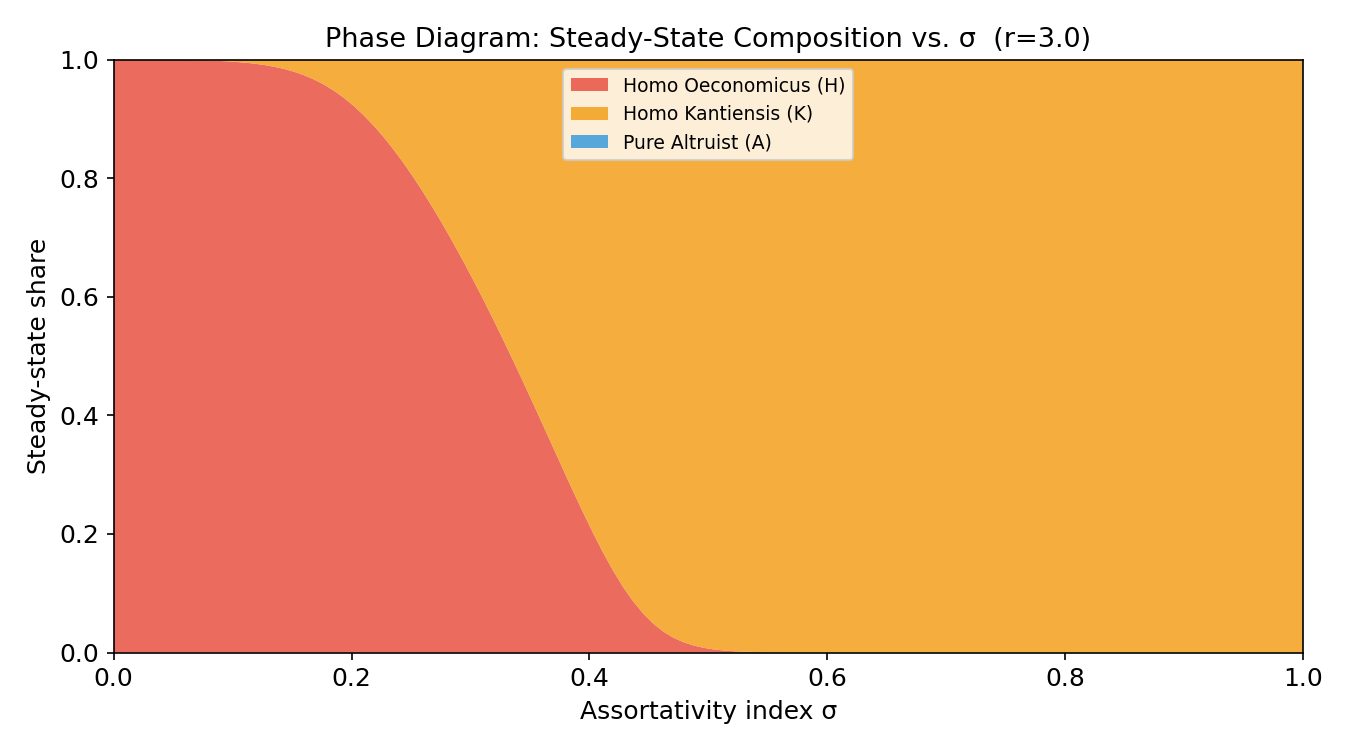
\includegraphics[width=0.85\textwidth]{Code/pgg_phase.png}
    \caption{Steady-state population composition as a function of assortativity $\sigma$ (stacked area chart). The Pure Altruist (A) maintains zero share throughout.}
    \label{fig:phase}
\end{figure}

The phase diagram reveals a clear transition structure:
\begin{itemize}
    \item $\sigma \lesssim 0.25$: H nearly completely dominant; K share close to zero.
    \item $0.25 \lesssim \sigma \lesssim 0.50$: gradual transition; K share rises as $\sigma$ increases, H share falls.
    \item $\sigma \approx 0.35$: approximate crossing point; shares roughly equal.
    \item $\sigma \gtrsim 0.50$: K becomes the near-sole stable type; H share rapidly approaches zero.
    \item A (Pure Altruist): share equals zero for all $\sigma \in [0,1]$.
\end{itemize}

The transition is S-shaped rather than abrupt: near the critical point, fitness differentials are smallest, so the transition proceeds most slowly.

\subsection{Simplex Phase Portrait}

Figure~\ref{fig:simplex} plots trajectories in the three-type simplex from eight distinct initial conditions under each of the four $\sigma$ values.

\begin{figure}[H]
    \centering
    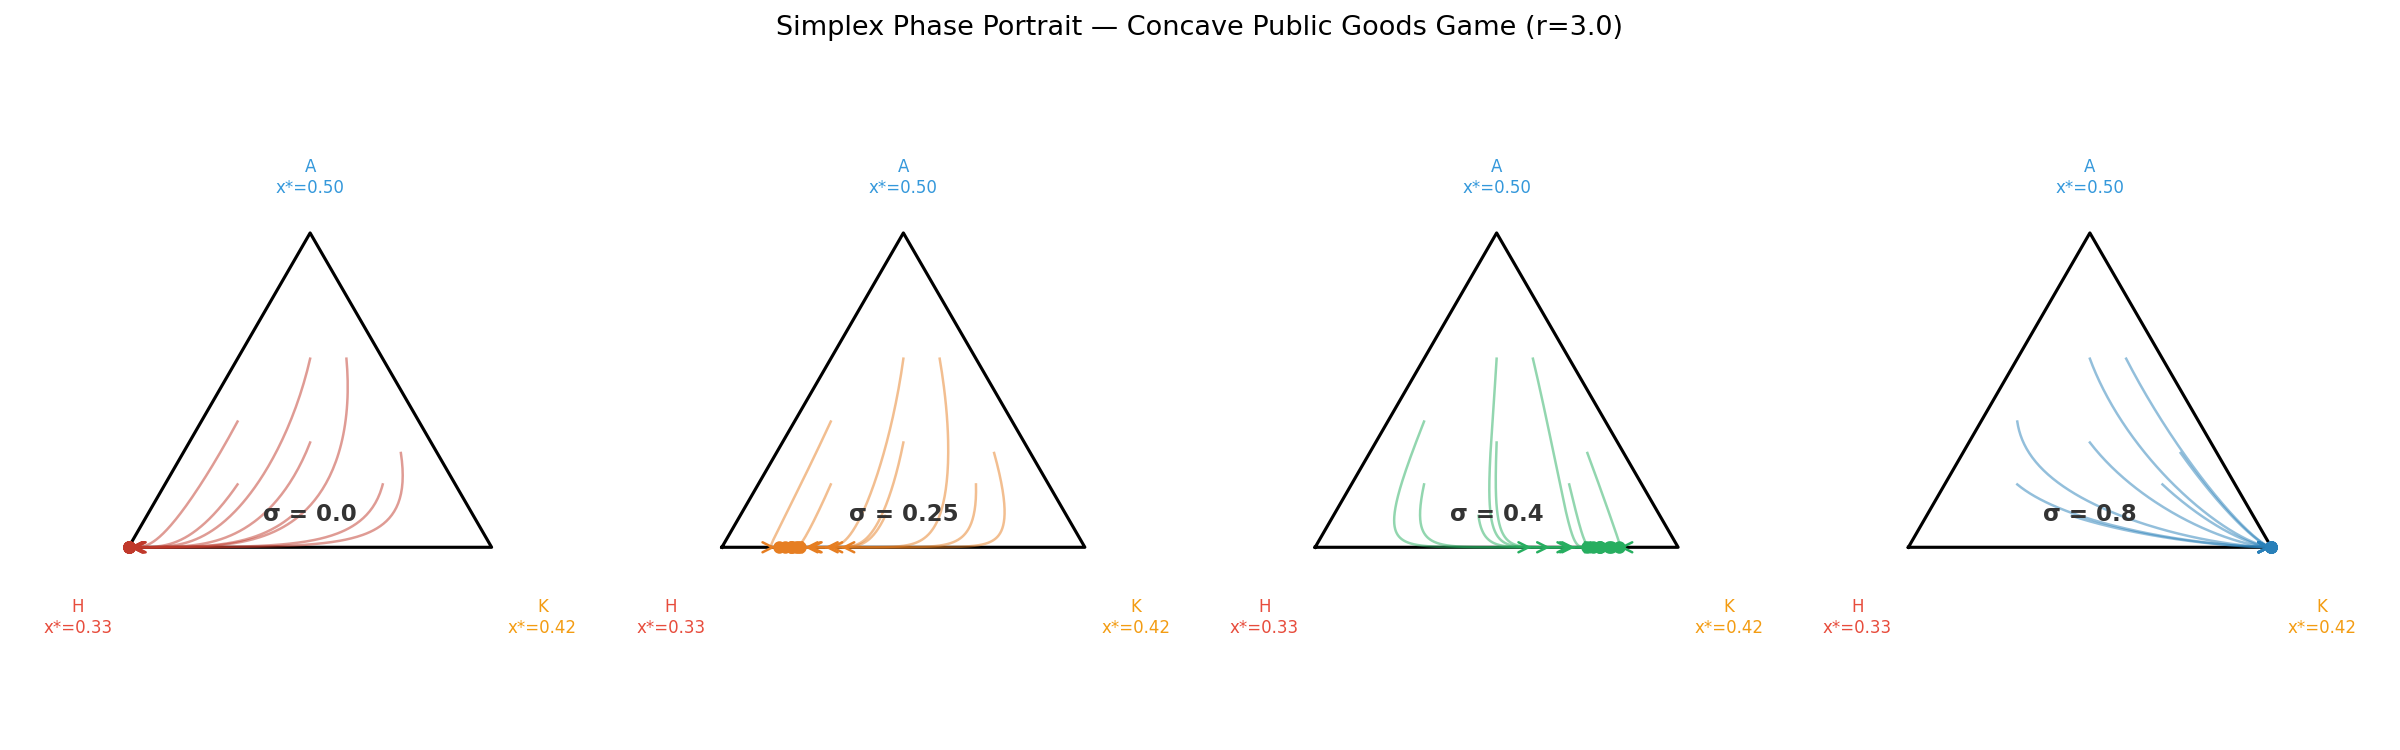
\includegraphics[width=\textwidth]{Code/pgg_simplex.png}
    \caption{Simplex phase portrait. Vertices H, K, A represent full dominance by each type. Trajectories originate from diverse initial compositions; arrows indicate direction of motion; dots mark attractors.}
    \label{fig:simplex}
\end{figure}

\begin{itemize}
    \item \textbf{$\sigma = 0.0$:} all trajectories converge to vertex H (global attractor). The A share vanishes first along all paths, then H eliminates K along the H-K edge.

    \item \textbf{$\sigma = 0.25$:} the attractor migrates to an interior point on the H-K edge (H $\approx 63\%$, K $\approx 37\%$). A is rapidly absorbed regardless of initial position.

    \item \textbf{$\sigma = 0.40$:} the attractor is an interior point on the H-K edge at (K $\approx 79\%$, H $\approx 21\%$). Several trajectories exhibit a ``detour'' toward the H vertex before reversing---a signature of the near-critical transient dynamics visible in Figure~\ref{fig:population}.

    \item \textbf{$\sigma = 0.80$:} all trajectories converge rapidly to vertex K (global attractor). The basin of attraction covers the entire simplex.
\end{itemize}

The A vertex is never an attractor and no trajectory approaches it, confirming that pure altruism is globally unstable under every matching regime.

%-----------------------------------------------------------------------
\section{Discussion}\label{sec:discussion}
%-----------------------------------------------------------------------

\subsection{Why Pure Altruism Fails: The Over-contribution Trap}

The Pure Altruist's elimination is not a consequence of the specific utility form chosen; it reflects a structural property of the concave public goods game. The altruist's equilibrium contribution $x_A^* = 1/2$ exceeds the social optimum $x_K^* = (2r-1)/4r$ for all $r > 1$. In a game with diminishing marginal returns, any contribution beyond the social optimum generates public benefit worth less than its private cost. The altruist thus inflicts an efficiency loss on herself \emph{that does not translate into commensurate benefit for the partner}.

More precisely, for any pair of types $(i, j)$:
$$\pi(x_A^*, x_j^*) < \pi(x_K^*, x_j^*) \quad \forall\, j,\, \forall\, \sigma.$$
This uniform dominance of K over A in material payoff is what drives A's elimination regardless of the population composition or matching structure.

The result points to a broader principle: \textbf{altruism and social efficiency are not the same thing}. Over-contribution is the symmetric counterpart of under-contribution (free-riding): both are deviations from the social optimum, in opposite directions. An altruistic preference that pushes contributions beyond the efficient level is not more beneficial to society than a selfish preference that pulls contributions below it; both misalign individual choice with collective welfare.

\subsection{Homo Kantiensis: Efficiency Through Moral Reasoning}

Homo Kantiensis dominates at high assortativity because its strategy coincides with the social optimum. This is not coincidental: in a symmetric concave game, the Kantian criterion---``choose $x$ to maximise $\pi(x,x)$''---is exactly equivalent to the social planner's problem of maximising aggregate welfare $2\pi(x,x)$. The Kantian agent reaches the social optimum \emph{not} by computing it directly, but by asking a moral question whose answer happens to be the socially efficient one under the specific payoff structure.

This connection between Kantian morality and social efficiency is specific to this class of games. It provides a microfoundation for why Kantian reasoning might be selected over both self-interest and pure altruism: not because it is intrinsically virtuous, but because it implements the correct allocation rule in a world with diminishing returns to cooperation.

The stability of Homo Kantiensis is nonetheless contingent on assortativity: its advantage over Homo Oeconomicus requires sufficiently frequent like-type encounters. This is consistent with the general result of \citet{AlgerWeibull2013}, whose main theorem states that the evolutionarily stable preference is homo moralis with Kantian weight $\kappa^* = \sigma$. The three-type model presented here is a discrete-type illustration of that theorem at the two extreme points ($\kappa = 0$ and $\kappa = 1$) plus the altruistic benchmark.

\subsection{Homo Oeconomicus and the Role of Social Structure}

Homo Oeconomicus is not eliminated; it is evolutionarily optimal \emph{conditional on the social structure}. In anonymous, large-population settings ($\sigma \approx 0$), free-riding is the dominant strategy and self-interest prevails. The failure of Homo Oeconomicus at high $\sigma$ is not a failure of rationality but a failure of the social conditions that make self-interest payoff-maximising.

This implies that \textbf{the evolutionary stability of a preference type is not an intrinsic property of the preference but a joint property of the preference and the matching environment}. Institutional or structural changes that raise $\sigma$---tighter community structures, repeated interaction, third-party monitoring---can shift the evolutionarily stable outcome from Homo Oeconomicus to Homo Kantiensis without any change in individual preferences. Conversely, a move toward anonymous large-scale markets ($\sigma \to 0$) selects for self-interest even in a population that initially contained substantial Kantian types.

%-----------------------------------------------------------------------
\section{Conclusion}\label{sec:conclusion}
%-----------------------------------------------------------------------

We have constructed a three-type evolutionary model of preference diversity in a concave public goods game and shown the following:

\begin{enumerate}
    \item \textbf{Pure Altruism is evolutionarily unstable at all assortativity levels.} The Pure Altruist's equilibrium contribution exceeds the social optimum, resulting in a self-inflicted fitness penalty relative to Homo Kantiensis under every matching regime. This is an example of the general principle that altruism and efficiency do not coincide: over-contribution is as inefficient as free-riding, merely in the opposite direction.

    \item \textbf{The Homo Oeconomicus--Homo Kantiensis contest is decided entirely by the assortativity index $\sigma$.} Low assortativity ($\sigma < 0.35$) selects for free-riding; high assortativity ($\sigma > 0.35$) selects for Kantian efficiency. The phase transition occurs at approximately $\sigma \approx 0.35$ for the concave game with $r = 3$.

    \item \textbf{In the concave public goods game, the Kantian moral criterion implements the social optimum.} Homo Kantiensis's evolutionary advantage at high $\sigma$ is therefore equivalent to the social optimum being selected---a result with direct welfare implications. The evolutionary mechanism does not merely approximate the social optimum; it exactly reaches it.

    \item \textbf{The replicator dynamics are equivalent to a simple population-replacement rule.} Under the assumption that entry is proportional to current type composition and death is proportional to relative fitness disadvantage, the standard replicator equation arises as the continuous limit without further parametric assumptions.
\end{enumerate}

The three-type model confirms and illustrates the central insight of \citet{AlgerWeibull2013}: moral preferences are not evolutionarily fragile; they are evolutionarily stable precisely when the social matching structure provides sufficient within-type interaction. The broader message is that the question ``which preference wins?'' cannot be answered without specifying the environment---and in environments with high assortativity, it is the preference that coincides with social efficiency, not the preference that maximises own payoff or the preference that maximises others' payoff, that prevails.

\bigskip
\noindent\textit{A closing remark.} The symmetric structure of the result deserves emphasis: in a world of diminishing returns, evolution does not reward the most selfish agent or the most selfless agent, but the agent who contributes \emph{exactly the right amount}---no more, no less.

\bibliographystyle{plainnat}
\bibliography{references}

\end{document}
